\section{Lesson 1 — History and Why Mathematics Came In}

\subsection{Definition of Cryptography}

The word \textbf{cryptography} originates from the Ancient Greek words \textit{κρυπτός} (\textit{kryptós}, “hidden, secret”) and \textit{γράφειν} (\textit{graphein}, “to write”).  
Therefore, cryptography literally means \textit{“the art of writing in secret”}.

\textbf{Common misspellings:} Crypthography, Criptography, Kryptography.

Cryptography has always been deeply connected with the need for secure communication. For thousands of years, kings, queens, and generals have relied on efficient communication to govern their empires and lead their armies. However, they were also aware of the risks of interception: a single message falling into enemy hands could reveal state secrets or military plans.  

It was precisely this threat that led to the invention of \textbf{codes} and \textbf{ciphers} — techniques for disguising a message so that only the intended recipient can understand it. Over the centuries, this gave rise to an ongoing struggle between \textbf{code makers} and \textbf{code breakers}. The development of cryptography is thus a history of constant evolution between securing and revealing secrets.  
\begin{flushright}
\textit{(Source: Singh, \emph{The Code Book})}
\end{flushright}

\subsection{Terminology}

Before proceeding, it is important to distinguish between some essential terms used throughout the course:

\begin{itemize}
  \item \textbf{Code:} replaces entire words with other words or symbols (e.g., “attack at dawn” $\rightarrow$ “JUPITER”).
  \item \textbf{Cipher:} replaces individual letters according to a rule or pattern (e.g., a→b, b→c gives “attack at dawn” $\rightarrow$ “buubdl bu ebxo”).
  \item \textbf{Plaintext:} the original message, written in lowercase.
  \item \textbf{Ciphertext:} the encrypted message, written in uppercase.
\end{itemize}

In modern terminology, the words \emph{decoding} and \emph{deciphering} are used interchangeably. However, the term “code” is mostly obsolete today, as virtually all systems are ciphers.

\subsection{Classical Cryptography}

The earliest forms of cryptography are known as \textbf{classical ciphers}. These include simple substitution systems such as the \emph{Caesar cipher}, where each letter is replaced by another letter shifted by a fixed number of positions in the alphabet.  

\begin{figure}[h!]
\centering
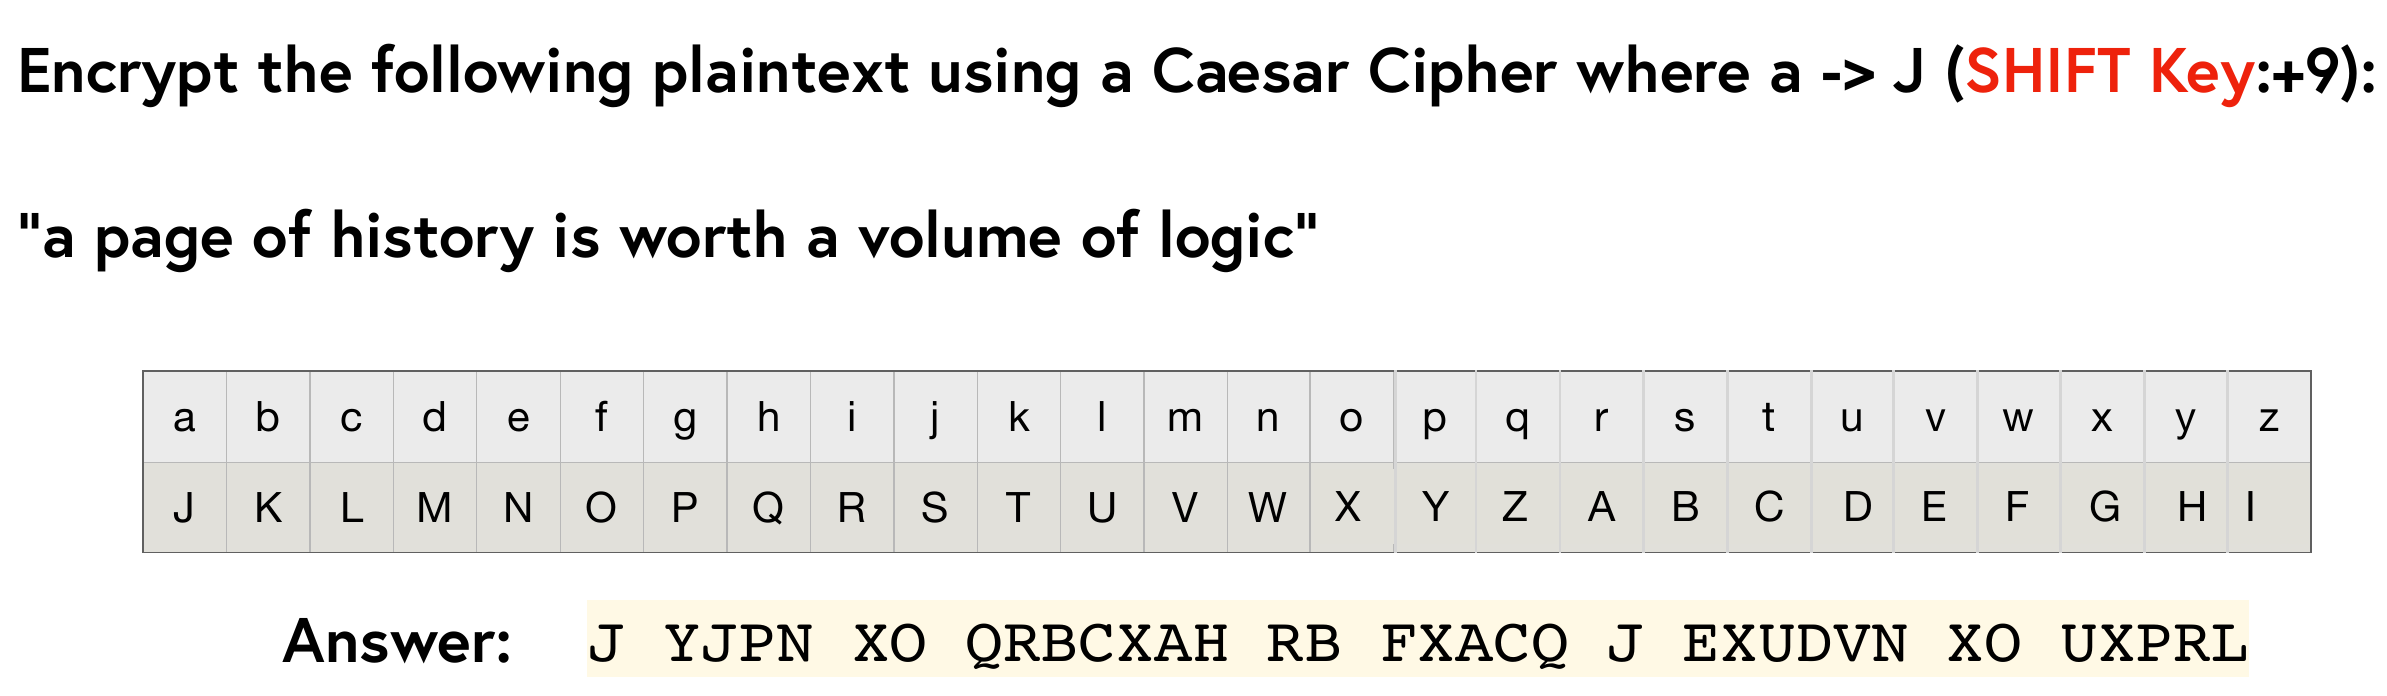
\includegraphics[width=0.7\textwidth]{Pictures/encrypt example.png}
\caption{An example of the Caesar cipher.}
\label{fig:caesar_cipher}
\end{figure}


\subsection{Example of Decryption}

Decrypt the ciphertext \texttt{DVVKZECFSSPRKKVE} assuming it was produced by a Caesar cipher.

\[
\text{Solution: } \texttt{meet in lobby at ten} \quad (\text{Key: } a \rightarrow R, \text{Shift } +17)
\]

This demonstrates that Caesar ciphers have only 26 possible keys — one for each possible shift of the alphabet.

\[
26! = 26 \times 25 \times \cdots \times 2 \times 1
\]

\[
\approx 4.03 \times 10^{26} \text{ possible rearrangements}
\]

Although this seems like a huge number, modern computation shows that brute force attacks on simple substitution ciphers are trivial for computers.

\subsection{Monoalphabetic Substitution Ciphers}

The \textbf{Caesar cipher} is just a special case of a more general class of ciphers called \textbf{monoalphabetic substitution ciphers}.  
In a monoalphabetic cipher, each letter of the alphabet is replaced by another letter or symbol, but the substitution rule remains fixed throughout the entire message.

While the Caesar cipher admits only 26 possible ciphers (one for each shift value), a full monoalphabetic substitution can be any permutation of the 26 letters of the alphabet. Hence, the total number of possible keys is:

\[
26! = 26 \times 25 \times \cdots \times 2 \times 1 = 403{,}291{,}461{,}126{,}605{,}635{,}584{,}000{,}000
\]

This number is astronomically large. If we were to try all combinations using a modern supercomputer performing $10^{18}$ operations per second, a complete brute-force attack would still require approximately \textbf{13 years} to finish.  
This demonstrates that a \emph{brute force} approach is not practical for monoalphabetic substitution ciphers.

\subsection{The First Known Cryptanalyst: Al-Kindi}

The first known description of a method for decrypting monoalphabetic substitution ciphers dates back to the 9th century.  
An Arab polymath named \textbf{Al-Kindi} wrote a treatise titled \textit{“A Manuscript on Deciphering Cryptographic Messages”}, discovered in 1987, which introduced the concept of \textbf{frequency analysis}.

\begin{quote}
Between 800 and 1200 AD, Arab scholars experienced a remarkable period of scientific and mathematical progress, while Europe was still in the Dark Ages.  
It was during this period that Al-Kindi developed the foundations of cryptanalysis — the art of breaking ciphers — centuries before similar methods appeared in Europe.
\end{quote}

\subsection{Frequency Analysis in English Texts}

The key idea of frequency analysis is that in any given language, letters do not appear with equal probability.  
In English, for example, the most common letters are:

\[
\text{e, t, a, o, i, n, s, h, r, d, l, u, m, w, c}
\]

A graphical representation of letter frequencies typically shows a sharp peak for “e”, which occurs in about 12\% of all text, followed by “t”, “a”, and “o”.

In addition to single letters, certain pairs of letters (called \textbf{digrams}) also appear more frequently than others.  
The most common digrams in English include \texttt{th}, \texttt{he}, and \texttt{in}.

\[
\begin{aligned}
\texttt{th} &\rightarrow 3.87\% \\
\texttt{he} &\rightarrow 3.69\% \\
\texttt{in} &\rightarrow 2.36\%
\end{aligned}
\]

\subsection{Decrypting Using Frequency Analysis}

A ciphertext produced by a monoalphabetic substitution can be attacked by comparing the frequency of letters in the ciphertext with the known frequency distribution of the English language.

For instance, if the letter “T” appears most frequently in the ciphertext, it is reasonable to hypothesize that it represents the plaintext letter “e”.  
By iteratively testing and refining these hypotheses — including frequent digrams such as “th” and “he” — one can gradually reconstruct the plaintext message.

This process, though slow by hand, is extremely efficient for modern computers, which can automatically compare statistical patterns of letters, bigrams, and trigrams.

\subsection{Example: Decrypting a Long Ciphertext}

Consider the following ciphertext:

\begin{verbatim}
LIVITCSWPIYVEWHEVSRIQMXLEYVEOIEWHRXEXIPFEMVEWHKVSTYLXZIXLIKIIXPIJVSZEYPE...
\end{verbatim}

By analyzing the frequencies of letters, digrams, and trigrams, and gradually mapping the most common ciphertext letters to their English counterparts, we can reveal the underlying plaintext.  

The final decoded message reads:

\begin{quote}
\textit{“This course aims to introduce you to the principles and techniques of securing computers and networks, focusing on Internet security. You will learn both theoretical and practical aspects of cryptography, algorithms, and real-world security protocols.”}
\end{quote}

This illustrates how frequency analysis alone is sufficient to break monoalphabetic ciphers — proving that no cryptography is better than bad cryptography.

\section{Unit 2 — Modern Cryptography: Polyalphabetic Ciphers}

\subsection{Introduction to Polyalphabetic Ciphers}

After centuries of monoalphabetic systems, cryptographers sought new methods to prevent attacks based on frequency analysis.  
The most famous innovation was the \textbf{Vigenère cipher}, invented around 1550 by \textbf{Giovan Battista Bellaso} and later misattributed to Blaise de Vigenère.

The idea was to apply multiple Caesar ciphers in sequence, each with a different shift value.  
These shifts are determined by a keyword that repeats cyclically across the message.

\[
\text{Example: Key } (2,5,4,7)
\]

Each letter of the plaintext is shifted by a different amount depending on its corresponding key value.

\[
\texttt{t h i s i s a s e c r e t}
\]

This sequence of varying shifts was once believed to make the cipher \textbf{unbreakable}, since the same plaintext letter could be encrypted differently depending on its position.

\subsection{Breaking the Vigenère Cipher}

Although it was considered secure for centuries, the Vigenère cipher was eventually broken through clever analysis.  
One of the first systematic methods was developed by \textbf{Friedrich Kasiski} in the 19th century.

The first step in breaking a Vigenère cipher is to determine the \textbf{key length}.  
This can be done by searching for repeating patterns of letters within the ciphertext.

\[
\text{Example: The sequence “VHX” appears multiple times.}
\]

By noting the distances between these repetitions, we can find that the gaps are often multiples of the key length.

\[
\begin{aligned}
133 - 1 &= 132 = 2^2 \times 3 \times 11 \\
172 - 133 &= 39 = 3 \times 13 \\
190 - 172 &= 18 = 2 \times 3^2 \\
280 - 190 &= 90 = 2 \times 3^2 \times 5
\end{aligned}
\]

The most common factors among these distances (3 and 6) suggest that the key length is likely 3.

\subsection{Frequency Analysis per Key Position}

Once the key length is known, the ciphertext can be divided into groups — each corresponding to a single Caesar cipher applied with a different shift.  
For example, if the key length is 3, letters at positions 1, 4, 7, 10, ... form the first group; positions 2, 5, 8, 11, ... form the second; and so on.

Each group can then be analyzed independently using classical frequency analysis.  
This allows us to identify the shift used for that specific part of the key.

\[
\text{Example: For the first group, the best match occurs when } a \rightarrow C \text{ (shift +2).}
\]
\[
\text{For the second group: } a \rightarrow A \text{ (no shift).}
\]
\[
\text{For the third group: } a \rightarrow T \text{ (shift +19).}
\]

Hence, the estimated key is \textbf{2–0–19}.

\subsection{Revealing the Plaintext}

By reversing the encryption using the key (2–0–19), the following plaintext emerges:

\begin{quote}
\textit{“The method used for the preparation and reading of coded messages is simple in the extreme and, at the same time, impossible to translate unless the key is known. The ease with which the key may be changed is another point in favor of this system.”}
\end{quote}

Although this was impressive for its time, after World War I the use of the Vigenère cipher declined sharply.  
It became clear that using the same key for long messages made the cipher vulnerable — and using one key per message was impractical.

\subsection{Historical Context: Codebreakers and the Evolution of Cryptography}

Since the 16th century, every major state has employed teams of \textbf{codebreakers}.  
History has shown that \emph{no cipher is better than a bad cipher}.  
A famous example is \textbf{Mary, Queen of Scots}, who was executed in 1587 after her encrypted letters were intercepted and deciphered by English cryptanalysts.

By the early 1900s, communication technologies such as the telegraph and radio outpaced the security of existing cipher methods.  
This allowed many secret wartime messages to be intercepted and decoded, with significant strategic consequences.  
For example, the decryption of the \textbf{Zimmermann Telegram} by British intelligence directly influenced the United States’ decision to enter World War I.

\section{Unit 3 — Cipher Machines}

\subsection{The Rise of Cryptographic Machines (1920–1970)}

With the spread of radio and telegraph communications in the early twentieth century, nations faced a new challenge: how to keep their messages secret while transmitting them over open airwaves.  
Traditional manual ciphers were no longer sufficient, and the need for \textbf{mechanical cryptographic devices} arose.

These machines automated complex substitutions and transpositions, making it possible to encrypt and decrypt messages much faster and more securely.

\subsection{The Enigma Machine}

One of the most famous cryptographic machines in history is the \textbf{Enigma}, invented by the German engineer \textbf{Arthur Scherbius} in 1918.  
Initially, the device was offered for commercial purposes but failed as a business product (its cost was equivalent to around \$30,000 today).  
Eventually, the German Army adopted it, purchasing thousands of units for military communication.

Enigma can be thought of as a \textbf{sophisticated letter scrambler}. Each key press triggered a chain of electrical substitutions determined by the internal configuration of mechanical rotors.

\subsection{The Rotors Mechanism}

The Enigma machine used three rotors, each containing a full 26-letter wiring permutation.  
When a letter key was pressed, current flowed through these rotors, and the letter was replaced by another.

After each key press, the first rotor rotated by one position.  
When it completed a full rotation (26 steps), the second rotor advanced by one step, and after the second made a full turn, the third moved as well — much like an odometer.  
This mechanism ensured that the same plaintext letter was encrypted differently each time it appeared in the message.

\[
\text{If you press the same key twice, two different letters appear!}
\]

Later versions allowed the operator to choose any three rotors among five available, further increasing complexity.  
The encryption setting depended on both the chosen rotors and their starting positions.

\subsection{The Reflector and the Plugboard}

To increase confusion, Enigma included a \textbf{reflector}, which sent the signal back through the rotors on a reverse path.  
This feature made encryption and decryption symmetrical: the same machine setup could be used for both processes.

In addition, the \textbf{plugboard} (German: \emph{Steckerbrett}) allowed the swapping of up to six pairs of letters before and after the rotor encryption.  
For instance, swapping \{A, D\} or \{B, U\} effectively inverted those letters at both input and output, adding yet another layer of complexity.

\[
\text{Signal path: } \text{Key} \rightarrow \text{Plugboard} \rightarrow \text{Rotors} \rightarrow \text{Reflector} \rightarrow \text{Rotors} \rightarrow \text{Plugboard} \rightarrow \text{Lampboard}
\]

\subsection{Configuration Space of Enigma}

The total number of possible Enigma configurations can be estimated as follows:

\begin{itemize}
  \item Each rotor has 26 positions, and there are 3 rotors in use $\Rightarrow 26^3 = 17,576$ settings.
  \item Rotors can be selected and arranged in order from a set of 5 $\Rightarrow 5 \times 4 \times 3 = 60$ combinations.
  \item Plugboard connections: typically 6 pairs of swapped letters, out of 26 $\Rightarrow \dfrac{26!}{14! \times 2^6} = 100{,}391{,}791{,}500$ possibilities.
\end{itemize}

Hence, the total number of possible configurations is approximately:

\[
72 \times 17{,}576 \times 100{,}391{,}791{,}500 \approx 2 \times 10^{17}
\]

This astronomical number made brute-force decryption impossible with the technology of the time.  
Even with a modern supercomputer performing $10^{18}$ operations per second, such an attack would still take many minutes — something unimaginable in the 1940s.

\subsection{Cracking Enigma — The Polish Breakthrough}

Despite its apparent strength, the Enigma machine contained exploitable weaknesses.  
In 1932, Polish mathematician \textbf{Marian Rejewski}, together with \textbf{Jerzy Różycki} and \textbf{Henryk Zygalski}, began working on the German cipher system.  
Using both mathematical reasoning and intelligence from German defectors, they discovered the internal rotor wirings.

At the time, each German message started with a \textbf{message key} — a three-letter sequence indicating the rotor starting position — which was encrypted twice using the same daily key.  
For example, if the operator chose the message key “ULJ”, the transmitted text might begin with its encrypted form “PEFNWZ”.

This repetition provided critical patterns that Rejewski could analyze mathematically.  
By studying these patterns and their \textbf{cycles}, he inferred information about the machine’s internal configuration.

\subsection{The Plugboard Problem and Rejewski’s Catalog}

The plugboard added about $10^{12}$ additional combinations, but Rejewski discovered that the overall \textbf{structure of chains and links} in the Enigma permutations remained the same regardless of plugboard settings.  
This insight allowed him to build a massive catalog of all possible cycle structures, dramatically reducing the search space.

It took about a year to compile this catalog for all possible rotor orders (only 3 rotors were in use at that time).  
Once completed, it enabled the Polish team to determine the daily key in minutes.

As a result, German communications were readable from \textbf{1934 onward}, long before the outbreak of World War II.

\subsection{Turing and the British Bombe}

In 1938, the Germans modified Enigma, increasing the number of rotors and plugboard pairs, which made the Polish method impractical.  
The mathematician \textbf{Alan Turing}, working at Bletchley Park in the United Kingdom, extended Rejewski’s ideas and built an electro-mechanical machine called the \textbf{Bombe}.

The Bombe exploited predictable message headers — such as the word “WEATHER” — to test possible rotor configurations and recover the keys much faster.

Recruitment for British codebreakers often involved solving complex crosswords published in the \textit{Daily Telegraph}, illustrating the strong link between linguistic skill and logical reasoning.

\subsection{The Lorenz Cipher and the Birth of the Computer}

For high-level communications between Hitler and his generals, the Germans used a far more complex machine: the \textbf{Lorenz SZ40}.  
The British cryptanalyst \textbf{Max Newman} designed a new electronic machine, called \textbf{Colossus}, to break Lorenz-encrypted messages.

Colossus, built in 1943, used over 1,500 electronic valves and was \textbf{programmable}, making it the first true digital computer.  
Its flexibility allowed it to adapt to different cryptographic problems, not just a single cipher type.

However, after the war, all Colossus machines were destroyed, and the knowledge of Enigma’s decryption remained secret until the 1970s.  
Consequently, the invention of the computer was officially credited to \textbf{Eckert and Mauchly} in 1945 with their ENIAC machine.

\section{Unit 4 — Modern Cryptography (1970– )}

\subsection{From Mechanical to Digital Cryptography}

The advent of electronic and digital computers in the 1970s completely changed the landscape of cryptography.  
Computers made it possible to both \textbf{encrypt} and \textbf{decrypt} messages at high speed — but also made many traditional ciphers vulnerable to brute-force attacks.

In the digital era, each letter, number, or symbol is converted into a binary sequence using \textbf{ASCII} encoding.  
For instance:
\[
\text{A} = 01000001, \quad \text{B} = 01000010, \quad \text{C} = 01000011
\]
This representation enables the encryption process to operate directly on bit sequences instead of alphabetic characters.

\subsection{Lucifer and the Birth of DES}

In 1971, \textbf{IBM} developed one of the first complex computer-based ciphers, called \textbf{Lucifer}.  
It was based on a combination of \textbf{substitution} and \textbf{transposition} operations — concepts inherited from classical cryptography but implemented digitally.

Lucifer eventually evolved into the \textbf{Data Encryption Standard (DES)}, which became the U.S. federal encryption standard and is still used in various legacy systems today.

Both Lucifer and DES are examples of \textbf{symmetric encryption systems}, meaning that the same secret key is used for both encryption and decryption.

\subsection{The Problem of Private Keys}

The fundamental weakness of symmetric ciphers lies in \textbf{key distribution}.  
For secure communication, both parties must share the same secret key — but transferring this key safely is not trivial.

During World War II, for example, the German military had to distribute entire \textbf{books of daily keys} to all Enigma operators.  
This posed enormous logistical and security challenges.

Even in peacetime, organizations faced difficulties ensuring that every communicating pair had exchanged a private key without interception.  
This limitation became one of the major driving forces behind the invention of modern cryptography.

\subsection{The Idea of Public Keys}

A natural question emerged:  
\begin{quote}
\textit{How can two people, Alice and Bob, communicate securely if an eavesdropper (Eve) can intercept all their messages, and they have no pre-shared key?}
\end{quote}

A simple analogy helps illustrate the problem.  
Imagine that Alice wants to send Bob a secret placed inside a box:

\begin{enumerate}
  \item Alice locks the box with \textbf{her own lock} (only she has the key) and sends it to Bob.
  \item Bob cannot open it, so he adds \textbf{his own lock} to the box and sends it back.
  \item Alice removes her lock and returns the box to Bob.
  \item Bob now removes his lock and retrieves the secret.
\end{enumerate}

This thought experiment, called the \textbf{double-lock protocol}, suggests that secure exchange might be possible without sharing keys.  
However, when implemented with mathematical ciphers, this fails because encryption and decryption operations are not necessarily commutative — i.e., order matters.

\subsection{Two Keys: One Private, One Public}

The conceptual breakthrough was to separate the key used for encryption from the one used for decryption.

\begin{itemize}
  \item Each person possesses a \textbf{public key} that can be freely shared with anyone.
  \item Each person also holds a \textbf{private key} known only to themselves.
\end{itemize}

If Alice wants to send a secret to Bob, she encrypts her message using \textbf{Bob’s public key}.  
Only Bob’s private key can decrypt it — even Alice cannot reverse the process.

This idea was first conceived by \textbf{Whitfield Diffie} and \textbf{Martin Hellman} at Stanford University in 1976, as described in their seminal paper \emph{“New Directions in Cryptography”}.

\subsection{The Diffie–Hellman Key Exchange}

The \textbf{Diffie–Hellman (DH) key exchange} protocol allows two parties to generate a shared secret key over an insecure channel using modular arithmetic.

Its security relies on the mathematical difficulty of computing discrete logarithms modulo a large prime number.

In simple terms:
\begin{itemize}
  \item Alice and Bob agree publicly on two numbers: a large prime $p$ and a base $g$.
  \item Alice chooses a private random number $a$ and computes $A = g^a \bmod p$.
  \item Bob chooses a private random number $b$ and computes $B = g^b \bmod p$.
  \item They exchange $A$ and $B$ publicly.
  \item Both can now compute the shared secret:
  \[
  K = g^{ab} \bmod p = (g^a)^b \bmod p = (g^b)^a \bmod p
  \]
\end{itemize}

An eavesdropper can see $p$, $g$, $A$, and $B$ — but recovering $a$ or $b$ (and thus $K$) is computationally infeasible for sufficiently large primes.

\subsection{The Digital Signature Problem}

While Diffie–Hellman solves the key exchange problem, it does not guarantee authentication.  
Alice has no proof that she is communicating with Bob and not with an attacker impersonating him — a scenario known as a \textbf{Man-in-the-Middle (MITM) attack}.

To address this, the concept of the \textbf{Digital Signature} was proposed.  
A digital signature is a mathematical scheme that allows a sender to prove the authenticity and integrity of a digital message.

Diffie and Hellman proposed the idea conceptually but could not find an efficient implementation — that would come only two years later.

\subsection{The RSA Cryptosystem}

In 1978, three researchers at MIT — \textbf{Ron Rivest}, \textbf{Adi Shamir}, and \textbf{Leonard Adleman} — developed the \textbf{RSA cryptosystem}, which implemented both public-key encryption and digital signatures.

RSA’s security is based on the mathematical difficulty of \textbf{factoring large integers} into their prime components.  
While multiplication of two primes is computationally simple, the inverse operation (factoring the product) is extremely hard for large numbers.

A similar idea had already been discovered in 1973 by the British mathematician \textbf{Clifford Cocks}, but it remained classified by GCHQ until 1997.

The RSA algorithm thus became the cornerstone of modern public-key cryptography, providing both \textbf{confidentiality} and \textbf{authentication} in digital communications.

\[
\text{Large number factoring: } N = p \times q \quad \Rightarrow \quad \text{Hard to find } (p, q)
\]

\subsection{Conclusion}

From the early Caesar cipher to modern RSA encryption, the evolution of cryptography shows a continuous interplay between secrecy, mathematics, and computation.  
As computing power grows, cryptography evolves to stay one step ahead — relying increasingly on abstract algebra, number theory, and complex mathematical problems.

\begin{center}
\textit{“History and why Mathematics came in Cryptography.” — End of Lesson 1}
\end{center}
